\chapter{Strumenti e tecnologie}
\label{cha:intro}
\vspace{5mm}

\section{Tecnologie utilizzate in Open Air Museum}\vspace{5mm}

Indicherò le varie tecnologie utilizzate per l'attuale versione dell'applicativo.\vspace{5mm}

\subsection{Filemaker}\vspace{5mm}

Filemaker è una piattaforma per creare applicativi personalizzati votati alla categoria “gestionale” sviluppata da Apple. Open Air Museum utilizza questa tecnologia per creare l’interfaccia per la raccolta dati che verrà utilizzata da alcuni addetti comunali che appunto arricchiranno l’applicativo con i testi e i media provenienti da questo software. Tale applicativo è standalone e quindi slegato dall’applicativo lato server che espone le Api e l’importazione dei dati provenienti da questa soluzione deve essere fatta manualmente. Ciò comporta uno svantaggio non indifferente che preclude una scalabilità rapida del prodotto. La scelta di questa tecnologia era quella di avere il più rapidamente possibile un prodotto in grado di iniziare a raccogliere dati il prima possibile e qualunque altra soluzione, seppur migliore in un ottica futura, avrebbe impiegato maggior tempo di sviluppo.\vspace{5mm}

\subsection{Node Js}\vspace{5mm}

	Come descritto in precedenza, Node js è un runtime di Javascript al di fuori del browser.Tale programma, come dicuterò più avanti, utilizza Chrome V8\cite{V8} come motore per eseguire Javascript ed grazie ciò NodeJs è stato fornito di una suite di interfacce per la comunicazione con l'hardware. In particolare questa particolare implementazione viene indicata come I/O non bloccante\cite{AsincIO}. La particolarità di questa soluzione è che mette a disposizione una serie di Api a basso livello che permettono di utilizzare la scheda di rete e quindi di avviare server TCP e HTTP oltre che accesso al file system quindi lettura e scrittura su disco. In Open air museum questo framework è utilizzato per costruire il lato server ed esporre una serie di Api Http Rest che permettono la fruizione dei dati. Tutti i media, quindi audio e immagini vengono serviti anch’essi da questa piattaforma che oltre a questo gestisce anche l’autenticazione degli utenti e la gestione degli stessi. \vspace{5mm}
	
	\subsection{Developer Tools}\vspace{5mm}
	
	Per sviluppare questo progetto le tecnologie che sono state utilizzate sono state dettate principalmente dalla necessità data dal sistema operativo che si voleva supportare o dalla tecnologia su cui si desiderava sviluppare. In particolare per lo sviluppo delle applicazioni mobili si è utilizzato XCode e Swift 4 come linguaggio per iOS mentre per Android si è utilizzato Android Studio e Java. La gestione delle dipendenze esterne si è optato per CocoaPods\cite{COCOA} per iOS mentre si è utilizzato Gradle 27.0.3 già incluso in Android Studio.\vspace{5mm}
	
	Per sviluppare la parte server si è utilizzato VisualStudio Code, un editor di testo con alcune funzionalità tra cui un implementazione grafica di un debugger per Nodejs.\vspace{5mm}
	
	L'intero progetto è stato metto sotto versioning control utilizzando Git come tecnologia e Bitbucket come applicativo di gestione delle repository. Si è adottato l'uso di creare tre repository separate per permettere una gestione più granulare delle impostazioni offerte da Bitbucket.
	
	\subsection{Modelli ER}\vspace{5mm}
		
	Il lato server utilizza come database relazionale MySql, che viene sfruttato attraverso un interfaccia Javascript che permette di connettersi al database  creando query inviandole mediante questa connessione ricevendo i dati in modo asincrono.
	Per quanto riguarda le due applicazioni, viene utilizzato sempre un database relazionale ma utilizzando SqLite come tecnologia; questo perché più leggero e adatto a essere eseguito su di un dispositivo dalle prestazioni ridotte.
	Lo schema relazionale per il lato server è il seguente:  \vspace{5mm}
	
\begin{figure}[h]
\centering
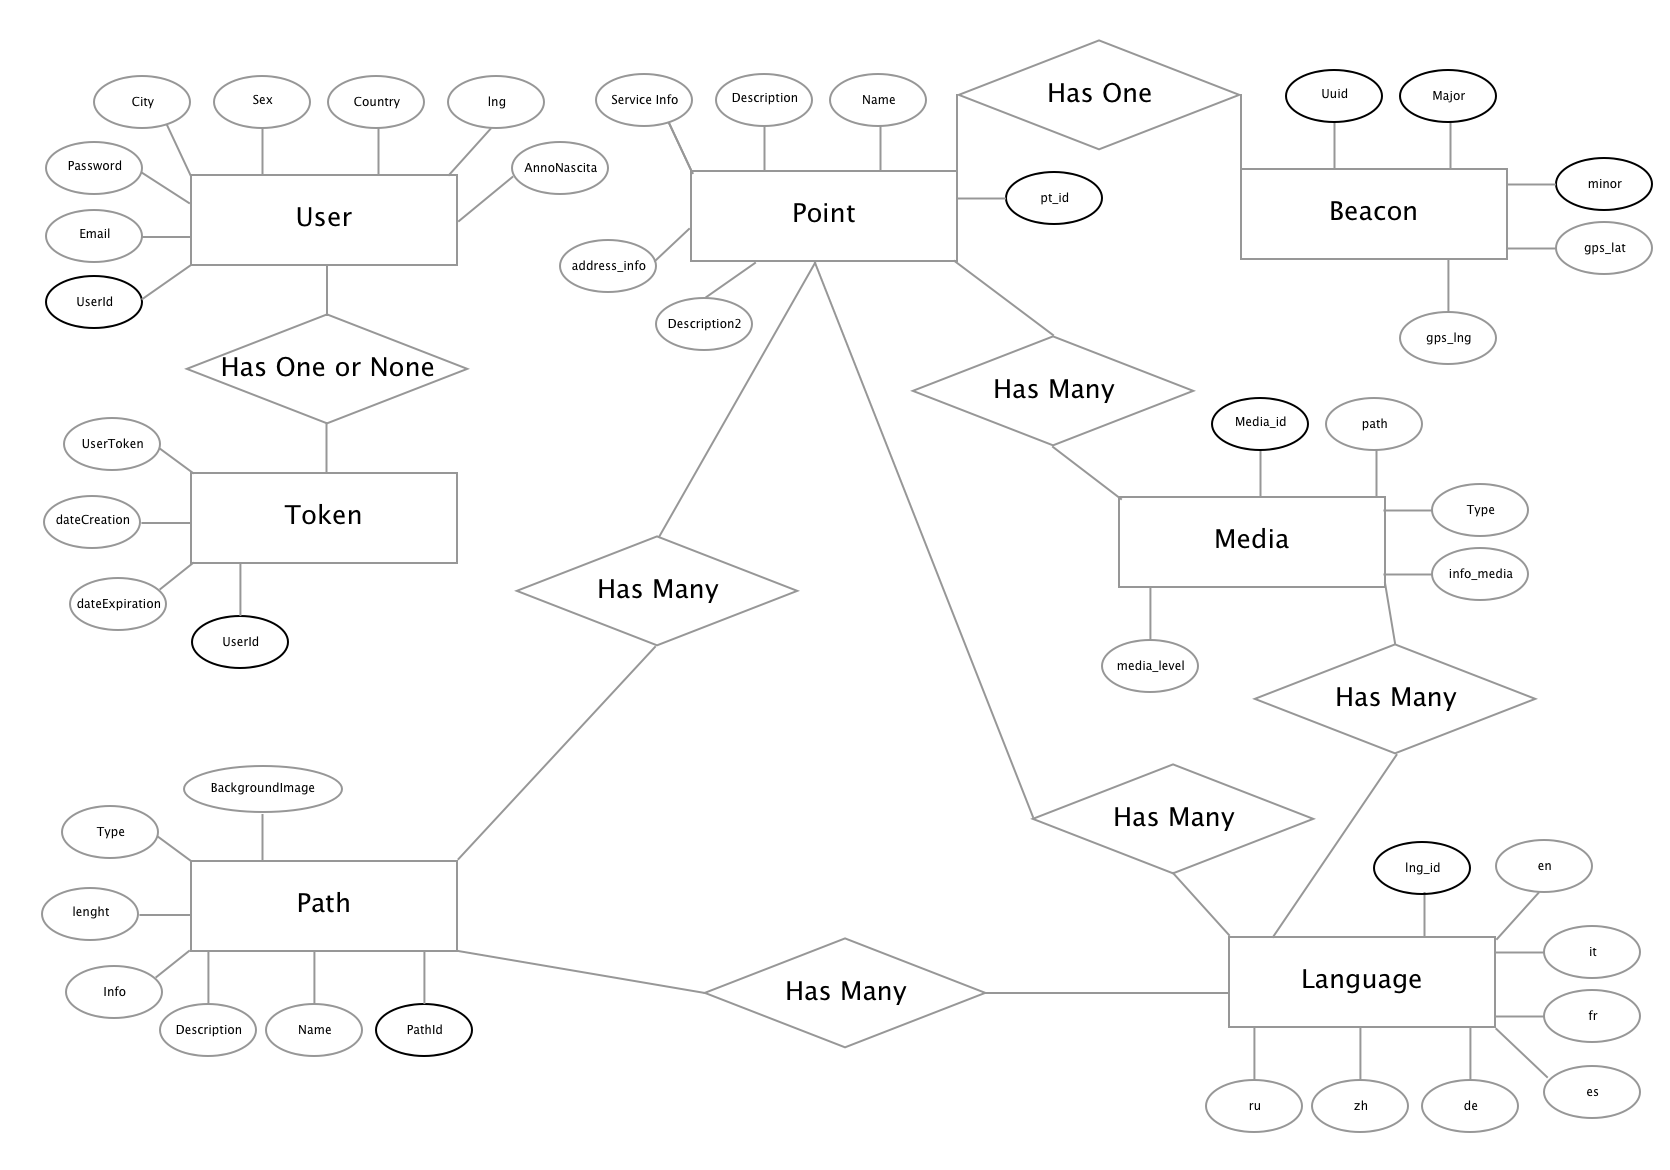
\includegraphics[width=0.9\textwidth]{images/erOld.png}
\caption{Schema ER vecchia versione server}
\end{figure}
\vspace{5mm}

Come si può vedere la gestione delle funzionalità multilingue avviene attraverso una relazione tra uno a molti tra i punti e i percorsi con la tabella 'language'. Questa tabella contiene tutti i testi per lingua supportata. Tale accorgimento è assente nello schema lato smartphone dato che, al cambiamento della lingua le nuove traduzioni verranno scaricate dalle Rest Api fornite a lato server. Lo schema relazionale per il lato mobile è il seguente:\vspace{30mm}

\begin{figure}[h]
\centering
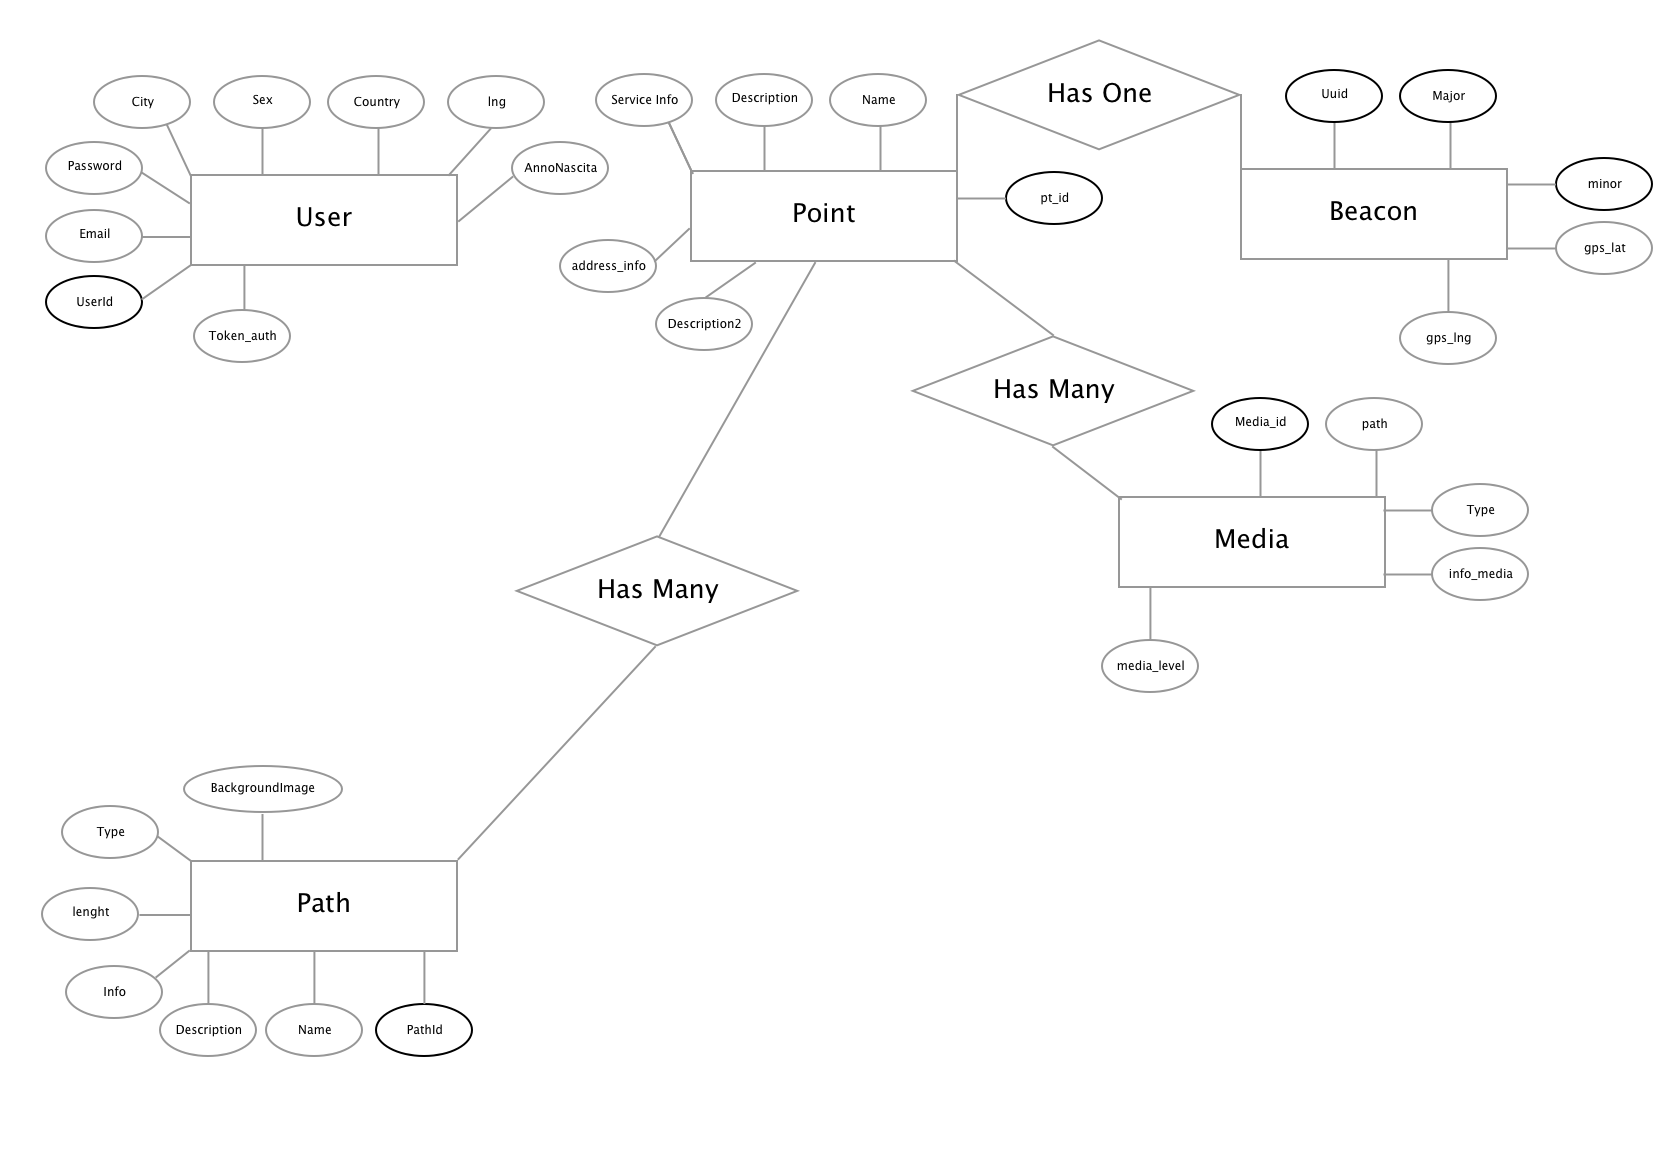
\includegraphics[width=0.9\textwidth]{images/erOldSpartphone.png}
\caption{Schema ER vecchia versione smartphone}
\end{figure}
\vspace{5mm}
	
\section{Tecnologie versione 2.0}\vspace{5mm}
Indicherò le varie tecnologie utilizzate per la nuova versione dell'applicativo ponendo particolare attenzione a che vantaggi portano.\vspace{5mm}

	\subsection{React}\vspace{5mm}

React\cite{React} è una Libreria Javascript per lo sviluppo di interfacce grafiche a componenti, permette lo sviluppo di single page application (SPA). Nella versione successiva l’applicativo che permette l’inserimento dei dati e dei media oltre alle descrizioni dei punti di interesse e dei percorsi è creata utilizzando questa tecnologia sfruttando un set di Api che il lato server fornisce. Questo centralizza la gestione dei dati in un unico luogo e cioè il server, tale approccio permette di utilizzare l'applicativo backend come unica fonte di verità senza dover gestire due prodotti separati come vi era in precedenza.\vspace{5mm}

	\subsection{Redux}\vspace{5mm}
	
	Redux è una libreria Javascript che permette di gestire lo stato applicativo come un unico oggetto statico, modificabile soltanto attraverso della azioni ben definite applicate ad esso. Ogni modifica viene fatta attraverso una funzione pura\cite{PureFunction} chiamata reducer che modifica a seconda dell'implementazione una parte specifica dello store. La firma di tale funzione prende due parametri, il primo è l'oggetto che rappresenta lo stato attuale dell'applicativo, il secondo è ciò che rappresenta l'azione che si sta compiendo. Tale azione dovrà sempre possedere una tipologia mentre può o non può avere un payload di dati che si riferiscono a quell'azione specifica. Ciò che ritornerà il reducer sarà un oggetto che diventerà il nuovo stato applicativo. Questa tecnologia è utilizzata per gestire i dati che gli applicativi mobile recupereranno dal server in modo predittivo e sicuro. Tale implementazione permette di evitare side effects\cite{SideEffects} nello stato applicativo facendo si che l'unica fonte di verità sia sempre affidabile e prevedibile. \vspace{5mm}
	
\begin{figure}[h]
\centering
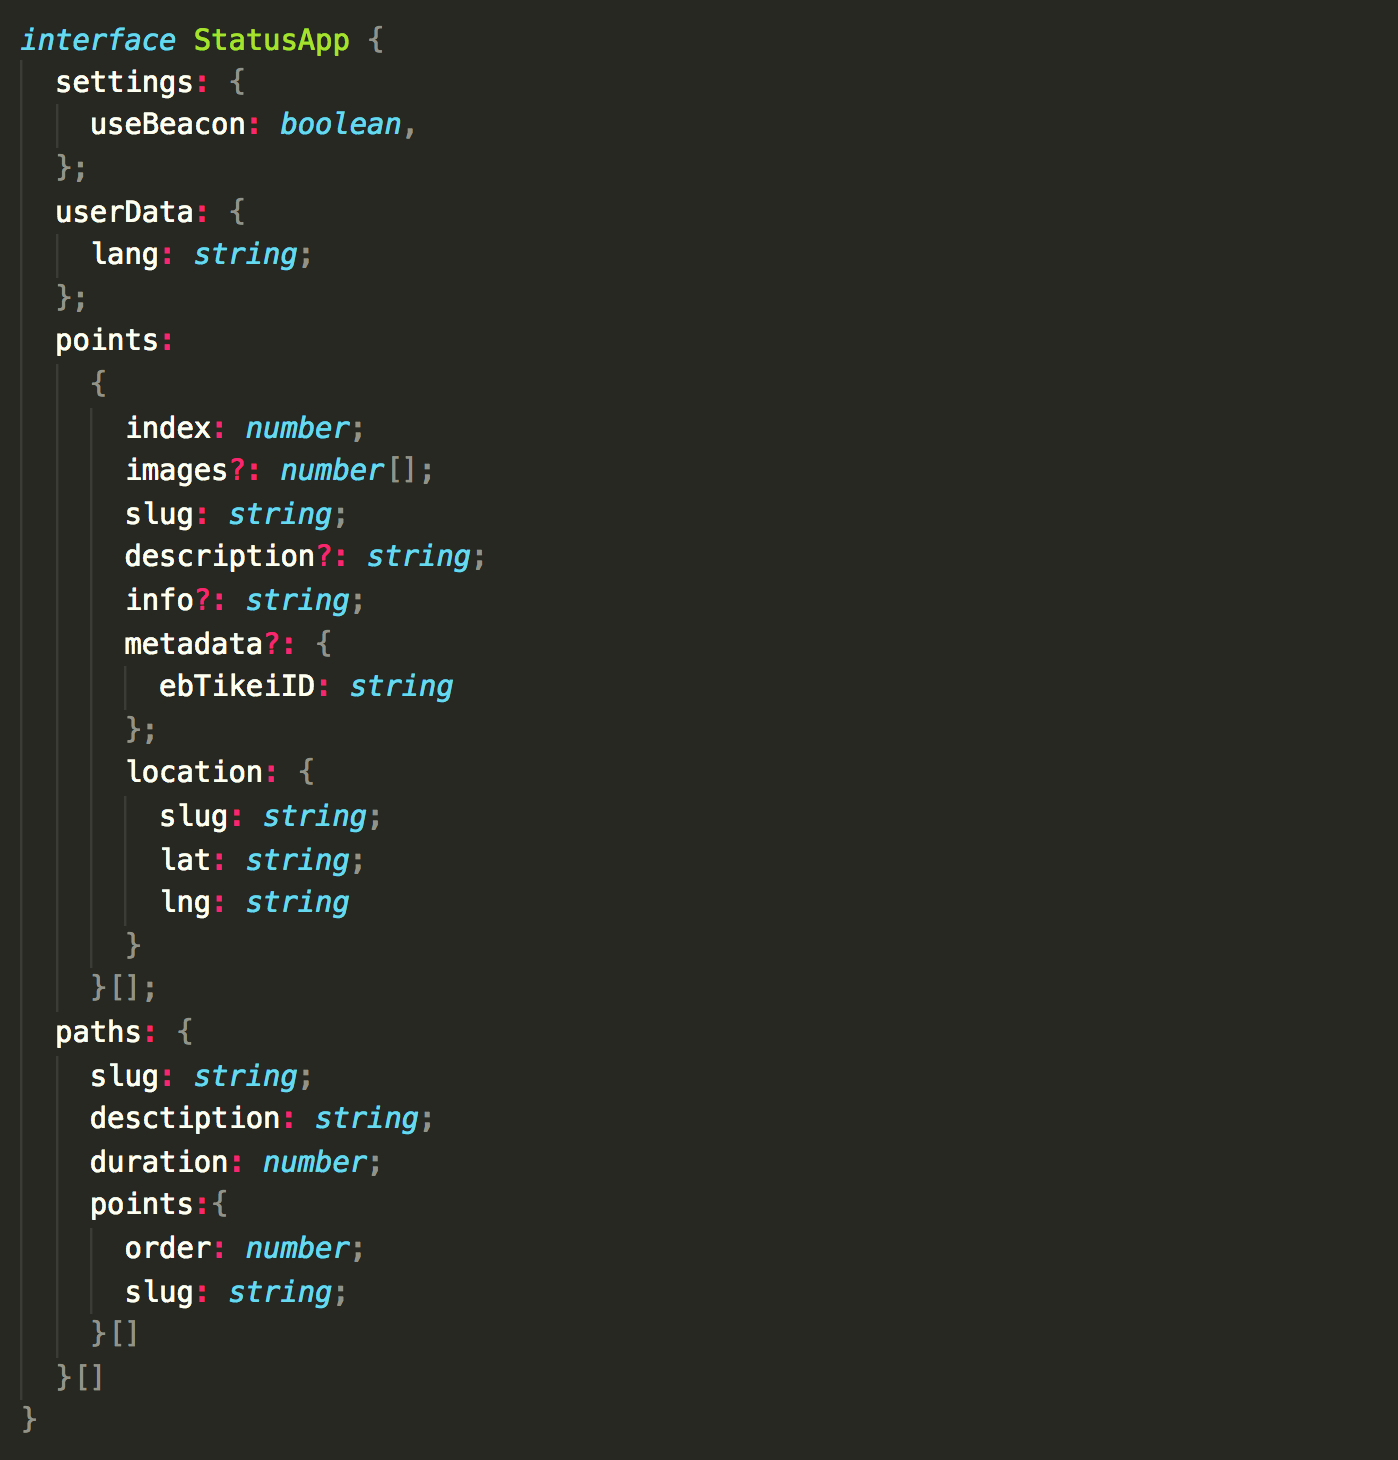
\includegraphics[width=0.7\textwidth]{images/store.png}
\caption{Interfaccia Store Redux}
\end{figure}
\vspace{5mm}

\subsection{React-Native}\vspace{5mm}

	React-Native è l'implementazione di React ma per l’ambiente nativo. Questa tecnologia verrà usata per creare l’interfaccia e la logica degli applicativi IOS e Android. Tale scelta infatti permette di condividere buona parte del codice tra le due piattaforme.\vspace{5mm}

\subsection{Express}\vspace{5mm}

	Express è l'implementazione del pattern middleware per Node Js. Tale framework permette di gestire con granularità il routing delle Api e da la possibilità di centralizzare la gestione degli errori. L'implementazione di tale pattern si riflette in un applicativo che esegue le computazioni attraverso una cascata di funzioni chiamate una dopo l'altra in ordine, ed ognuna di esse ha la facoltà di decidere se continuare la catena o interrompere la computazione. Questo permette di avere una struttura affidabile per gestire il routeing delle Rest api rendendo molto veloce e predittivo lo sviluppo.\vspace{5mm}

\subsection{SqLite}\vspace{5mm}

	SqLite è “File-based” database utilizzato lato server per il salvataggio delle informazioni fornite dagli utenti admin attraverso l’applicativo web per la raccolta dei dati. Tale scelta è stata fatta per la flessibilità di questa tecnologia che permette di gestire internamente all’applicativo la creazione dello stesso e non attraverso una dipendenza esterna. Questo è stato fatto per semplificare ulteriormente il deploy eliminando le necessità di aggiungere una configurazione ulteriore all’ambiente.\vspace{5mm}
	
	\subsection{Modello ER}\vspace{5mm}

Ora descriverò brevemente il nuovo schema logico dell'applicativo e come le varie tecnologie, tutte basate su Javascript interagiscono fra loro.
	
\begin{figure}[h]
\centering
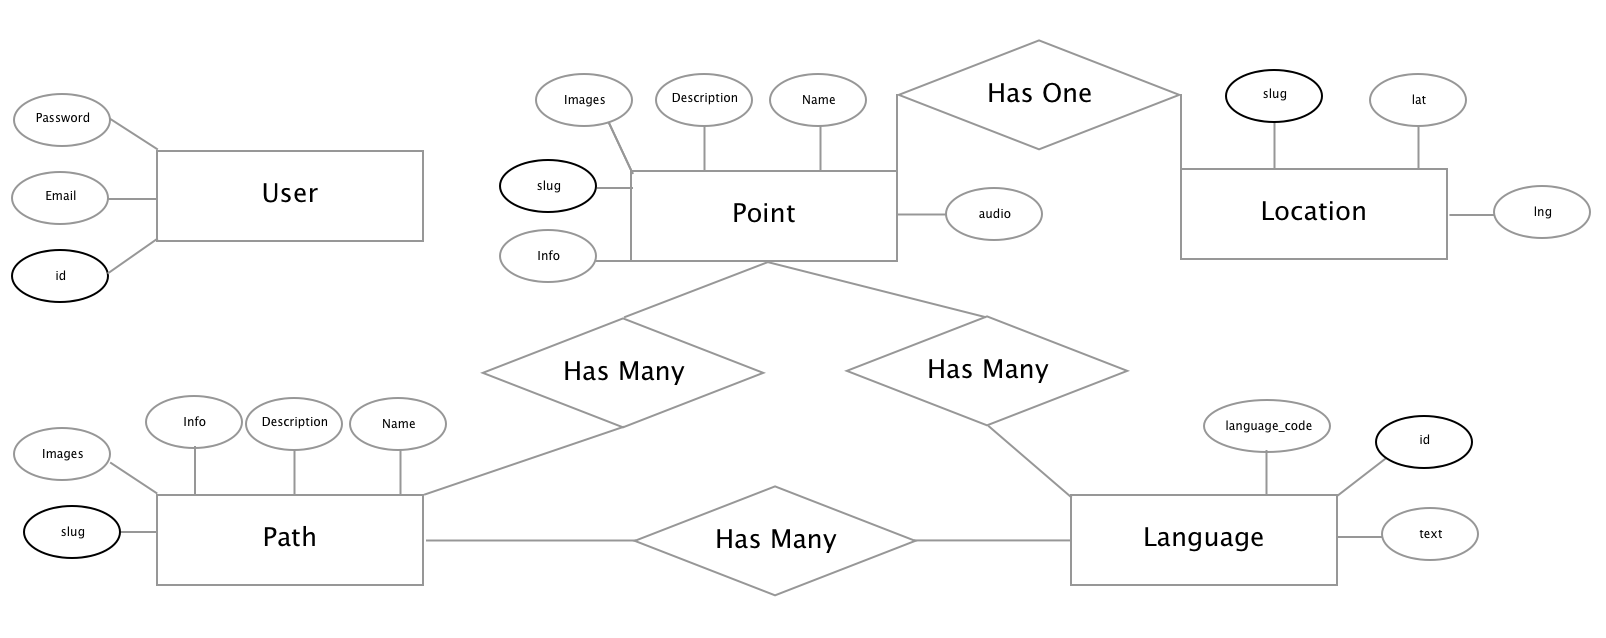
\includegraphics[width=0.9\textwidth]{images/erNew.png}
\caption{Schema ER nuova versione}
\end{figure}
	
	
\begin{figure}[h]
\centering
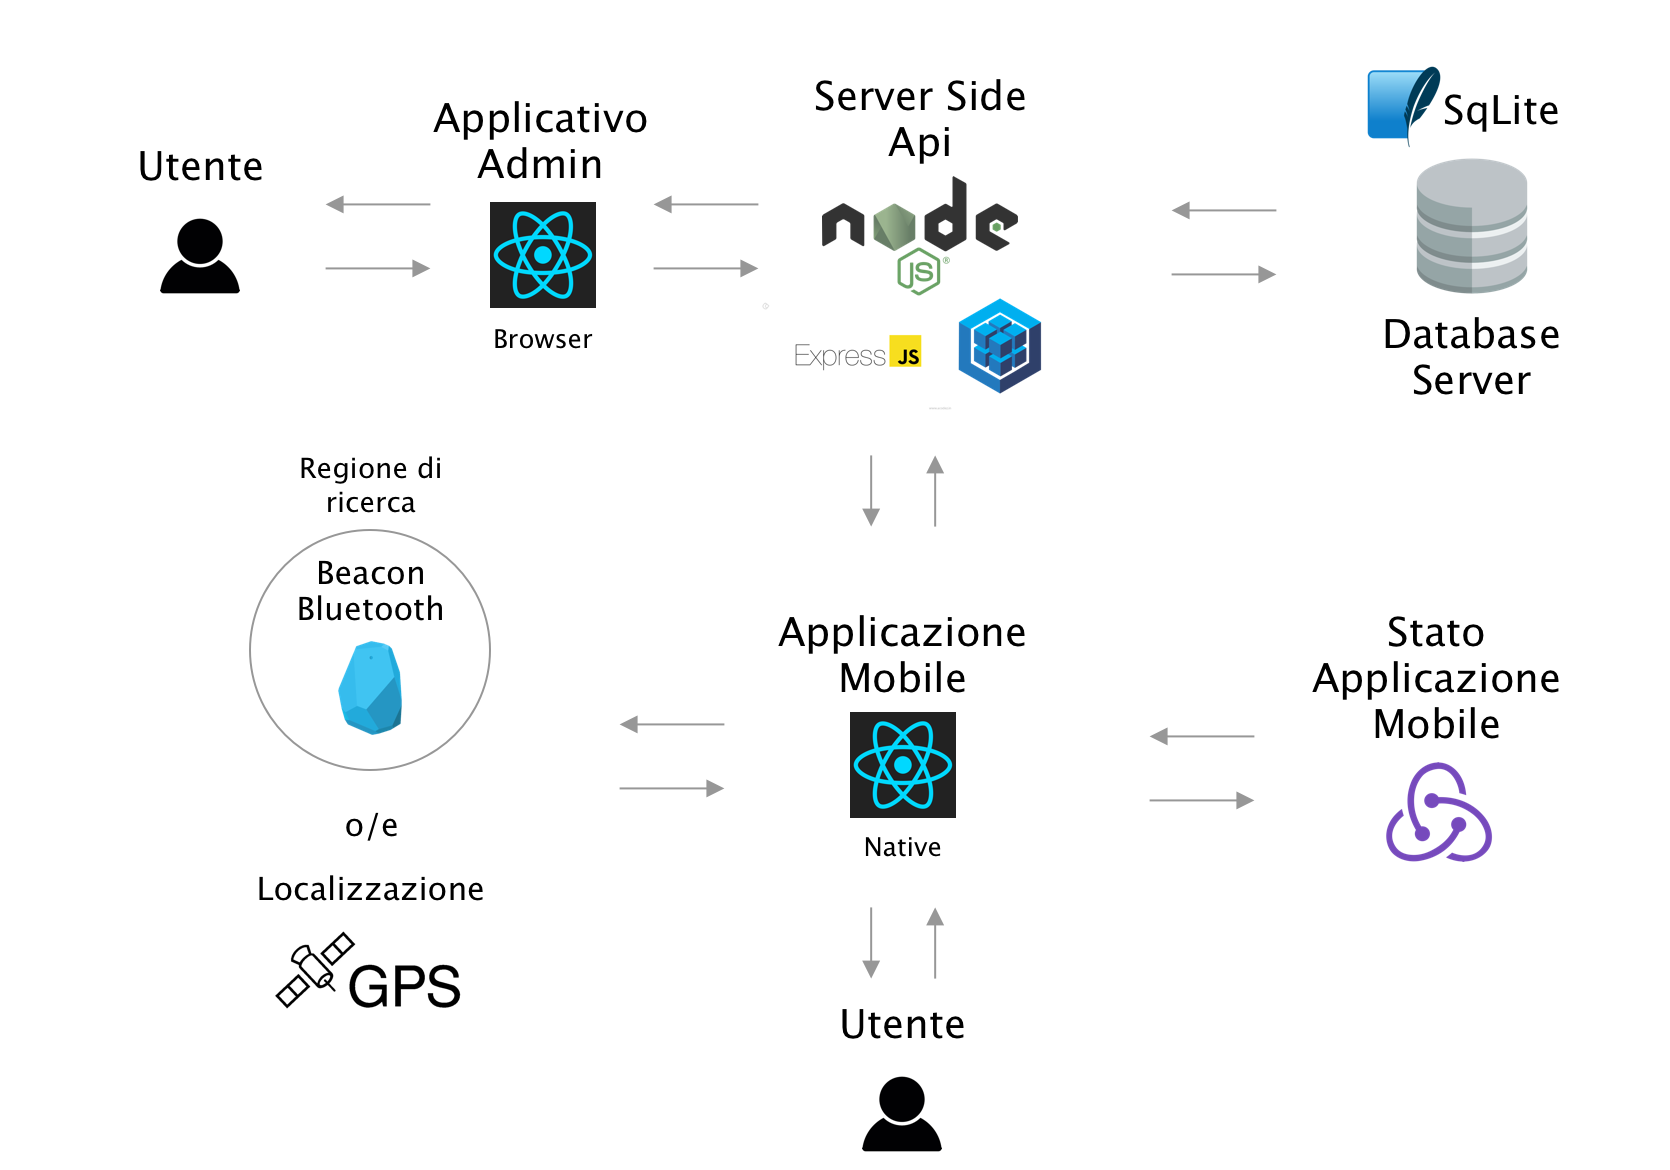
\includegraphics[width=0.9\textwidth]{images/stackAlakai.png}
\caption{Schema stack nuova versione}
\end{figure}

\vspace{5mm}Come si può vedere in figura 2.4 lo stack risulta meno complesso e vanta l'utilizzo di meno tecnologie per raggiungere le medesime funzionalità. Come si può notare i punti di interazione con la piattaforma sono gestiti da due applicativi basati entrambi su React, il primo è l'applicativo mobile che utilizza React-native mentre il secondo è la webApp admin. Entrambi questi applicativi ricevono input dall'utente ma il primo utilizza hardware esterno per arricchire la propria raccolta informazioni con la posizione dell'utente, ricevuta attraverso il gps o Beacon bluethoot. Tali applicativi interagiscono con il server mediante delle Rest Api che, come nella versione precedente, forniscono i dati sui punti e i percorsi; ma, in contrasto con l'applicativo prima del refactor, portano anche la configurazione impostata dall'applicativo admin in modo da adattarlo alle richieste di chi gestisce i punti e i percorsi. Tali dati vengono salvati in un database SqLite il cui unico punto di accesso è attraverso le api fornite dal server. \vspace{5mm}

Tale approccio garantisce che i dati siano sempre consistenti con quello che è l'applicativo server in modo da mantenere la struttura consistente con il versionamento del prodotto. Un ulteriore struttura per mantenere i dati è presente a lato mobile mediante Redux, questo è utile per poter salvare le configurazioni e mantenerle tali in modo consistente attraverso l'app in modo da creare una coesione tra tutti i componenti di React che necessitano di usufruire dei dati. Tale stato applicativo viene idratato attraverso le api Rest e quando questo non è possibile per mancanza di rete permette di utilizzare tramite React-native lo Storage locale del dispositivo come luogo di backup. Ogni mutazione dello stato applicativo viene infatti seguita da un operazione asincrona che ha lo scopo di salvare uno snapshot dello store nella memoria del dispositivo in modo da poter essere sempre consistente nel mostrare gli ultimi dati disponibili anche se il dispositivo risulta offline.\vspace{5mm}


